%%%%%%%%%%%%%%%%%%%%%%%%%%%%%%%%%%%%%%%%%%%%%%%%%%%%%%%%%%%%%%%%%%%%%%%%%%%%%%%%%%%%%%%%%%%%%%%%%%%%%%%%
%Andrea Favero
%10/09/2017
%Relazione progetto corso Programmazione ad Oggetti PAO1617
%%%%%%%%%%%%%%%%%%%%%%%%%%%%%%%%%%%%%%%%%%%%%%%%%%%%%%%%%%%%%%%%%%%%%%%%%%%%%%%%%%%%%%%%%%%%%%%%%%%%%%%%

\documentclass[10pt, a4paper]{article}

\usepackage[scaled]{helvet}

\usepackage[utf8]{inputenc}
\usepackage[T1]{fontenc}
\usepackage[italian]{babel}

\usepackage{xcolor}

\usepackage{graphicx}
\usepackage{fix-cm}
\newcommand{\bigsize}{\fontsize{35pt}{20pt}\selectfont}
\newcommand{\mediumsize}{\fontsize{30pt}{20pt}\selectfont}
\newcommand{\normsize}{\fontsize{15pt}{10pt}\selectfont}

\usepackage{float}

\definecolor{UniPD}{RGB}{155, 0, 20}

\usepackage[colorlinks=true]{hyperref}
\hypersetup{
	colorlinks=true,
	citecolor=black,
	filecolor=black,
	linkcolor=UniPD, % colore dei link interni
	urlcolor=Maroon  % colore dei link interniesterni
}

% permette di modificare i margini
\usepackage[top=3.1cm, bottom=3.1cm, left=2.2cm, right=2.2cm]{geometry}

\usepackage{blindtext}
\usepackage{scrextend}
\addtokomafont{labelinglabel}

%permette di simulare shell unix
\usepackage{suffix}
\newcommand{\shellcmd}[1]{\\\indent\indent\texttt{\footnotesize\$ #1}\\}
\WithSuffix\def\shellcmd*#1{\indent\indent\texttt{\footnotesize\$ #1}\\}
%%%%%%%%%%%%%%%%%%%%%%%%%%%%%%%%%%%%%%%%%%%%%%%%%%%%%%%%%%%%%%%%%%%%%%%%%%%%%%%%%%%%%%%%%%%%%%%%%%%%%%%%

\begin{document}
	
%%%%%%%%%%%%%%%%%%%%%%%%%%%%%%%%%%%%%%%%%%%%%%%%%%%%%%%%%%%%%%%%%%%%%%%%%%%%%%%%%%%%%%%%%%%%%%%%%%%%%%%%
	\begin{titlepage}
		\centering
		
		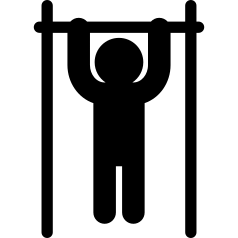
\includegraphics[width=50mm]{immagini/logo.png}
		\vspace*{50px}
		
		{\bigsize RELAZIONE\\}
		\vspace*{5px}
		{\bigsize PROGRAMMAZIONE\\}
		\vspace*{5px}
		{\bigsize AD OGGETTI\\}
		\vspace*{25px}
		
		{\mediumsize QONTAINER}
		\vspace*{30px}
		
		{\mediumsize Andrea Favero\\}
		\vspace*{5px}
		{\normsize Matricola: 1125545}
		\vspace*{30px}
		
		\includegraphics[width=50mm]{immagini/dip_mat.png}\\
		\vspace*{2.5px}
		{\normsize Tullio Levi Civita\\}
		\vspace*{20px} %tutto il resto va in fondo alla pagina
		{\mediumsize  Laurea in Informatica\\ }
		\vspace*{\fill}
		{\normsize Anno Accademico 2018/2019\\ }

\end{titlepage}
%%%%%%%%%%%%%%%%%%%%%%%%%%%%%%%%%%%%%%%%%%%%%%%%%%%%%%%%%%%%%%%%%%%%%%%%%%%%%%%%%%%%%%%%%%%%%%%%%%%%%%%%
{
% i link dei colori della table of contents diventano neri, togliamo da questi il colore UniPD
\hypersetup{hidelinks}
\tableofcontents
}
%%%%%%%%%%%%%%%%%%%%%%%%%%%%%%%%%%%%%%%%%%%%%%%%%%%%%%%%%%%%%%%%%%%%%%%%%%%%%%%%%%%%%%%%%%%%%%%%%%%%%%%%
%\begin{abstract}\end{abstract}
%%%%%%%%%%%%%%%%%%%%%%%%%%%%%%%%%%%%%%%%%%%%%%%%%%%%%%%%%%%%%%%%%%%%%%%%%%%%%%%%%%%%%%%%%%%%%%%%%%%%%%%%
\section{Ambiente di sviluppo}
\begin{itemize}
	\item{Sistema operativo: 
	    \begin{itemize}
	        \item Fedora GNU\textbackslash{Linux} 29
	        \item Ubuntu GNU\textbackslash{Linux} 19.04
	    \end{itemize}
	}
	\item {Compilatore:
	    \begin{itemize}
	        \item Fedora: g++ 8.3.1 20190223 (Red Hat 8.3.1-2)
	        \item Ubuntu: g++ 8.3.0
	    \end{itemize}
	}
	\item{Versione librerie Qt: 5.12.2}
\end{itemize}
\section{Ore impiegate:}
\begin{itemize}
	\item{analisi preliminare del problema: $2$}
	\item{progettazione ed implementazione model: $10$}
	\item{progettazione ed implementazione view: $34$}
	\item{apprendimento libreria Qt: $1$ (perché già imparata gli anni scorsi)}
	\item{relazione: $1$}
	\item{debug + testing: $2$}
	\item{totali: $50$}
\end{itemize}

\section{Scopo del progetto}
\emph{QONTAINER} è un'applicazione che permette agli atleti che praticano il nuoto, il ciclismo, la corsa
o il triathlon di tenere traccia dei loro allenamenti. Una volta inseriti i dati relativi alle loro prestazioni, 
essi possono vedere per ciascun allenamento quante calorie hanno bruciato, quanti sali minerali hanno consumato
e quanti grammi di peso hanno perso.

QONTAINER permette di inserire, modificare ed eliminare gli \emph{atleti} ed i loro \emph{allenamenti}.
Offre inoltre una funzionalità di ricerca che per un dato atleta visualizza i relativi allenamenti (tutti
oppure filtrati per sport) che soddisfano certe caratteristiche temporali (una certa data)
e prestazionali (\emph{i.e.}: il minimo ed il massimo numero di vasche a dorso che sono state fatte
durante un allenamento di nuoto).

Il programma utilizza due contenitori templatizzati, uno per gli atleti di tipo
\emph{Contenitore<std::shared\_ptr<Persona>>}, l'altro per gli allenamenti di tipo \emph{Contenitore<DeepPtr<Allenamento> >}.

\section{Descrizione delle gerarchie dei tipi usate}
Il progetto presenta tre tipi di gerarchie, una presente nella parte logica e due presenti in quella grafica.
\subsection{Gerarchia parte logica}
La gerarchia presente nella parte logica è totalmente indipendente dalla libreria \emph{Qt} ed utilizza solamente
la libreria standard del linguaggio C++. Tale gerarchia è presente nella figura sottostante.
\begin{figure}[H]
	\centering
	\def\svgwidth{.75\linewidth}
	\input{gerarchia.pdf_tex}
	\label{figure:gerarchia_allenamenti}
	\caption{Gerarchia parte logica}
\end{figure}
La classe base astratta virtuale polimorfa \emph{Allenamento} modella un generico
allenamento sportivo portato a termine da un atleta tenendo conto anche della data
e della durata in minuti. Il campo dati atleta è di tipo \emph{std::shared\_ptr<Persona>} perché
tutti gli atleti dell'applicazione sono memorizzati in un contenitore parametrizzato su
\emph{std::shared\_ptr<Persona>} che è un puntatore smart condiviso, in questo modo, quando un utente modifica un atleta non 
si crea alcuna discrepanza nei dati dei suoi allenamenti perché rimangono sempre tutti correlati a lui e non ai vecchi nome, 
cognome e sesso che aveva prima della modifica. 
Definisce i metodi virtuali:
\label{sec:metodi}
\begin{labeling}{alligator}
    \item[\textbf{$\sim$ Allenamento() = default}]
    \item[\textbf{std::string tipo() const = 0}] %//ritorna una stringa che rappresenta il tipo dell'allenamento
    \item[\textbf{Allenamento* clone() const = 0}] %//classico metodo di clonazione polimorfa
    \item[\textbf{unsigned int calorie() const = 0}]% //calorie consumate durante l'allenamento
    \item[\textbf{unsigned int grassoPerso() const = 0}]% //grammi di grasso perduti per via dell'allenamento
    \item[\textbf{unsigned int saliMinerali() const = 0}]% //sali minerali consumati
    \item[\textbf{bool operator==(const Allenamento\&) const}]
    \item[\textbf{bool operator>=(const Allenamento\&) const}]
    \item[\textbf{bool operator<=(const Allenamento\&) const}]
\end{labeling}
Le classi \emph{Nuoto}, \emph{Ciclismo} \emph{Corsa} e \emph{Triathlon} sono la concretizzazione della
classe \emph{Allenamento} da cui derivano. Le classi derivate fanno l'override di tutti i metodi virtuali
della classe base ad eccezione del distruttore dato che non ce n'è necessità.

Il metodo \textbf{calorie()} permette di sapere quante calorie ha bruciato l'atleta durante l'allenamento,
\textbf{saliMinerali()} quanti milligrammi di sali minerali sono stati consumati e \textbf{grassoPerso()} quanti grammi
di grasso sono ''andati perduti'' per via dell'allenamento.

\subsection{Gerarchie parte grafica}
La parte grafica è formata da due gerarchie, una (visualizzata nella figura sottostante) riguardante i \emph{delegate} 
utilizzati per disegnare a video i bottoni contenuti nelle \emph{QTableView} e che permettono di eliminare o modificare 
un allenamento oppure un atleta, l'altra (nella figura sottostante) riguardante i dialog utilizzati per
creare o modificare un certo allenamento.

\subsubsection{Gerarchia delegati}
La gerarchia dei delegati è composta dalla classe base \emph{DelegatoBottone} che eredita da
\emph{QItemDelegate} e fa l'override del distruttore virtuale e dei metodi \textbf{paint()}
(che si occupa di disegnare a video i bottoni) e \textbf{editorEvent()} (che gestisce
la pressione del mouse sui bottoni). Le due sottoclassi di \emph{DelegatoBottone} sono
\emph{DelegatoEliminazione} e \emph{DelegatoModifica}. La prima è il delegato che gestisce i
bottoni di eliminazione (di un atleta o un allenamento) e la seconda è il delegato che gestisce
i bottoni di modifica (di un atleta o un allenamento). Nessuna delle due fa l'override dei metodi
presenti nella classe base ma, vengono aggiunti semplicemente dei signal e degli slot
necessari per eliminare\textbackslash modificare un allenamento o un atleta.
\begin{figure}[H]
	\centering
	\def\svgwidth{.75\linewidth}
	\input{gerarchiaBottoni.pdf_tex}
	\label{figure:gerarchiaBottoni}
	\caption{Gerarchia parte logica}
\end{figure}

\subsubsection{Gerarchia dialog}
La gerarchia dei \emph{Dialog}, derivante da \emph{QDialog} ha lo scopo di fornire delle finestre
di dialogo finalizzate a permettere all'utente di aggiungere o modificare un allenamento.
La gerarchia controlla anche che i campi inseriti dall'utente siano validi e, nel caso si accettino le modifiche
apportate o che si inserisca un nuovo allenamento, modifica o inserisce l'allenamento nel contenitore e poi avverte
il model perché si aggiorni.
La classe base \emph{DialogAllenamento} non ha alcun motivo per essere istanziata e per questo definisce i metodi
virtuali puri \textbf{setLabelTitolo()}, \textbf{inserimentoAllenamento()} e \textbf{modificaAllenamento()} (questi ultimi
due sono slot).
\begin{figure}[H]
	\centering
	\def\svgwidth{.75\linewidth}
	\input{gerarchiaDialog.pdf_tex}
	\label{figure:gerarchiaDialog}
	\caption{Gerarchia delegati}
\end{figure}

\section{Utilizzo del codice polimorfo}
\subsection{Codice polimorfo classi allenamenti}
I metodi virtuali \hyperref[sec:metodi]{listati in precedenza} vengono richiamati come segue:
\begin{itemize}
    \item \textbf{tipo()}: riga $46$ della classe \emph{ModelTabellaAllenamenti};
    \item \textbf{clone()}: righe $32$, $37$, $49$ della classe \emph{DeepPtr};
    \item \textbf{calorie()}: riga $53$ della classe \emph{ModelTabellaAllenamenti};
    \item \textbf{grassoPerso()}: riga $55$ della classe \emph{ModelTabellaAllenamenti};
    \item \textbf{saliMinerali()}: riga $57$ della classe \emph{ModelTabellaAllenamenti};
    \item \textbf{operator>=}: righe $34$, $36$ della classe \emph{SortFilterProxyModelAllenamenti};
    \item \textbf{operator<=}: righe $34$, $36$ della classe \emph{SortFilterProxyModelAllenamenti};
    \item \textbf{operator==()}: riga $175$ della classe \emph{DialogTriathlon}, 
        $114$ della classe \emph{DialogCiclismo}, $111$ della classe \emph{DialogCorsa},
        $116$ della classe \emph{DialogNuoto};
\end{itemize}

\subsection{Codice polimorfo classi dialog}
Benché le classi della gerarchia reimplementano i metodi virtuali puri della classe base, non viene effettuata alcuna chiamata 
polimorfa perché tali metodi sono richiamanti solamente all'interno del costruttore della classe. Non c'è alcun motivo per
richiamarli al di fuori dato che servono solamente per impostare l'interfaccia grafica dei dialog, cosa che solitamente viene
fatta dai costruttori.
 
\section{Manuale utente}
\subsection{Creazione di un nuovo atleta}
La cosa da fare al primo avvio se non si sceglie di utilizzare i file forniti di default è  \emph{creare un nuovo atleta}.
Bisogna quindi andare sulla tab relativa agli atleti e cliccare sul bottone \textbf{Nuovo Atleta} in basso al centro, si aprirà
un dialog che permetterà di inserire i dati necessari alla creazione. Una volta creato l'atleta comparirà una nuova riga relativa ad esso
sulla tabella e cliccando sui bottoni \textbf{modifica} o  \textbf{elimina} si potrà  rispettivamente modificare o eliminare tale atleta.

\subsection{Creazione di un nuovo allenamento}
Quando nel sistema è presente almeno un atleta è possibile inserire un nuovo allenamento.
Per farlo bisogna spostarsi nella tab Allenamenti e cliccare sul bottone dello sport scelto situato in basso al centro.
Una volta fatto si aprirà un nuovo dialog che permetterà di istanziare un nuovo allenamento: bisogna selezionare l'atleta desiderato e la data, bisogna  immettere la durata in minuti e i milligrammi di sali minerali che sono stati assunti prima o dopo l'allenamento. Se si è scelto il nuoto
è necessario che l'atleta abbia nuotato almeno una vasca in uno qualsiasi dei tre stili, se si è scelto il ciclismo oppure
la corsa è necessario che abbia percorso almeno un km in una delle qualsiasi specialità disponibili. Per il triathlon che comprende nuoto, corsa e ciclismo sono necessarie le stesse cose.
Una volta creato l'allenamento comparirà sulla tabella una nuova riga relativa ad esso in cui, sono presenti dati calcolati in base alle informazioni immesse in fase di creazione.
Per rivedere tali informazioni o modificare l'atleta è sufficiente cliccare
sul bottone modifica, per eliminarlo basta cliccare su modifica.

\section{Ricerca}
È possibile effettuare la ricerca sugli allenamenti relativi ad \textbf{un} certo atleta. Per farlo bisogna spostarsi nella tab Ricerca (visualizzata nella figura sottostante) e selezionare l'atleta desiderato.
Esistono due tipi di ricerca, una generale che filtra tutti gli allenamenti 
di qualsiasi tipo fatti dall'atleta (bisogna selezionare il radio button \textbf{Atleta}) oppure quella relativa ai singoli sport (bisogna selezionare i radio button riguardanti gli sport).
Dopodiché è necessario inserire il range di tempo in cui si vogliono cercare gli allenamenti e anche il minimo ed il massimo valore relativo alle caratteristiche proprie degli sport.
Per ogni sport è necessario che il valore minimo di \textbf{almeno una} sua caratteristica (\emph{i.e.} il numero minimo di vasche a stile, rana o dorso se si prende in considerazione il nuoto) sia $\geq 1$.
Una volta completato l'inserimento cliccando sul bottone \textbf{Cerca} è possibile visualizzare i risultati filtrati a seconda dei dati immessi.

\begin{figure}[h]
    \caption{Schermata di ricerca}
    \centering
    \includegraphics[width=0.5\textwidth]{ricerca.png}
    \label{figure:gerarchiaDialog}
    \caption{Ricerca}
\end{figure}



\section{Formato file caricamento e salvataggio del contenitore}
Il programma utilizza dei file con estensione \emph{.xml} e opera sui file \emph{atleti.xml} ed \emph{allenamenti.xml}
che contengono rispettivamente gli atleti che vengono caricati sul contenitore relativo agli atleti e su quello 
relativo agli allenamenti. Per velocizzare la correzione del progetto al primo avvio viene offerta la possibilità di 
utilizzare dei file già pronti contenenti atleti ed allenamenti.

\section{Indicazioni di compilazione ed esecuzione}
La compilazione del progetto necessita del file QONTAINER-MV.pro.
Per compilare è necessario dare i comandi: \shellcmd{qmake}\shellcmd*{make}
Per avviare l'eseguibile basta dare il comando \shellcmd{./QONTAINER-MV}
%%%%%%%%%%%%%%%%%%%%%%%%%%%%%%%%%%%%%%%%%%%%%%%%%%%%%%%%%%%%%%%%%%%%%%%%%%%%%%%%%%%%%%%%%%%%%%%%%%%%%%%%
\end{document}
%%%%%%%%%%%%%%%%%%%%%%%%%%%%%%%%%%%%%%%%%%%%%%%%%%%%%%%%%%%%%%%%%%%%%%%%%%%%%%%%%%%%%%%%%%%%%%%%%%%%%%%%